
\section{Überblick}

\begin{frame}
  {Relationen und Prädikate}
  \pause
  \begin{itemize}[<+->]
    \item Verbsemantik und Valenz: semantische Rollen
      \Halbzeile
    \item Warum ist der Begriff \textit{Subjekt} überflüssig?
    \item Warum ist der Begriff \textit{Prädikat} problematisch?
    \item Wieviele Passive gibt es, und welche Verben sind passivierbar?
    \item Was sind direkte, indirekte und PP-Objekte?
    \item Und was sind Dativ- und PP-Angaben?
      \Halbzeile
    \item \alert{Valenzänderungen} und \alert{Valenzerweiterungen}
      \Halbzeile
    \item Gerade \alert{wegen} der Schwierigkeiten mit der Schulterminologie\\
      wird hier heute Wichtiges gelernt!
  %\begin{itemize}[<+->]
    \item \citet{Schaefer2018b}
  %\end{itemize}
  \end{itemize}

\end{frame}

\begin{frame}
  {Relationen?}
  \pause
  \begin{itemize}[<+->]
    \item \alert{Kategorien}
      \begin{itemize}[<+->]
        \item Wortklasse?
        \item Numerus
        \item Tempus
        \item Komparationsstufe
        \item Kasus?
          \Halbzeile
        \item \alert{für die jeweilige Einheit definiert}
      \end{itemize}
      \Halbzeile
    \item \alert{Relationen}
      \begin{itemize}[<+->]
        \item Subjekt, Objekt (zum Verb)
        \item Ergänzung\slash Angabe (zu einem Wort)
        \item Prädikat (eines Satzes?)
        \item Attribut (zu einem Nomen)
          \Halbzeile
        \item \alert{zwischen Einheiten definiert}
        \item \alert{erfordern oft bestimmte Kategorien}
      \end{itemize}
  \end{itemize}
  \pause
  \Halbzeile
  \rot{Relationen helfen, syntaktische Strukturen zu dekodieren.}
\end{frame}

\begin{frame}
  {Übrigens: grammatische Mittel und Bildungssprache}
  \pause
  Aus \citet{Feilke2012}\\
  \Halbzeile
  \pause
  \centering
  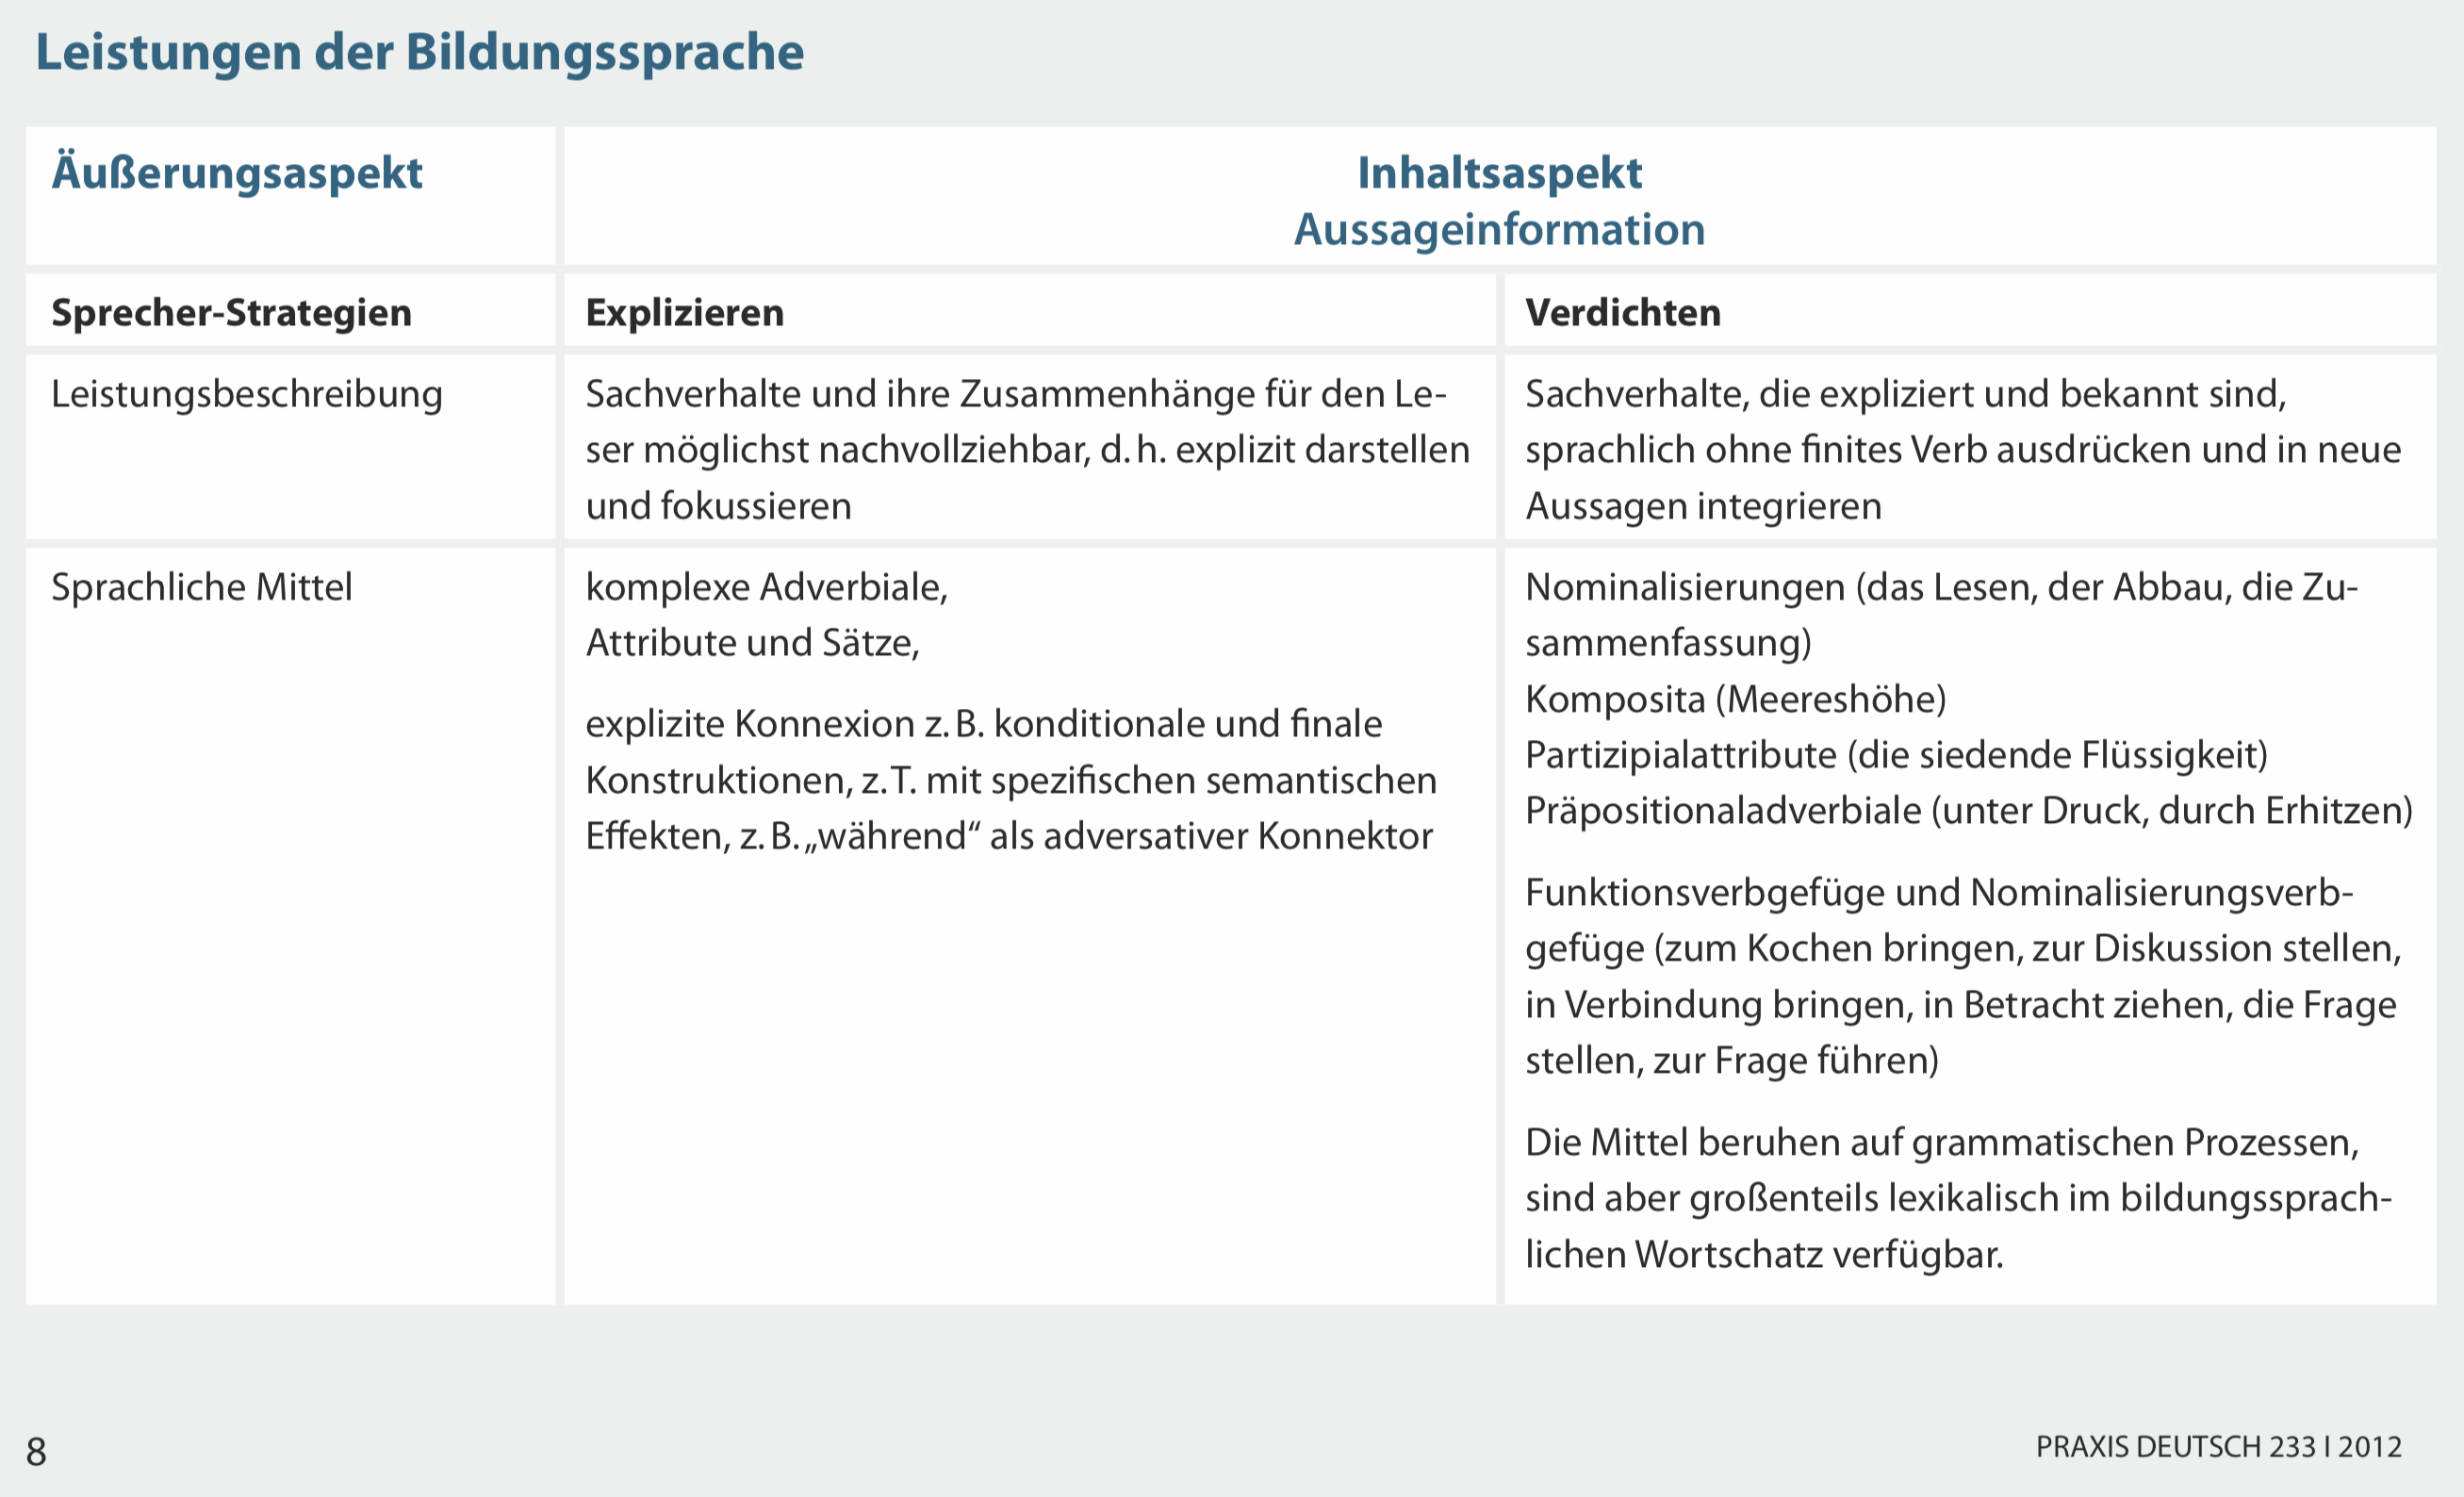
\includegraphics[width=0.8\textwidth]{\GRAPHPATH/feilke1}
\end{frame}


\begin{frame}
  {Übrigens: grammatische Mittel und Bildungssprache}
  Aus \citet{Feilke2012}\\
  \Halbzeile
  \centering
  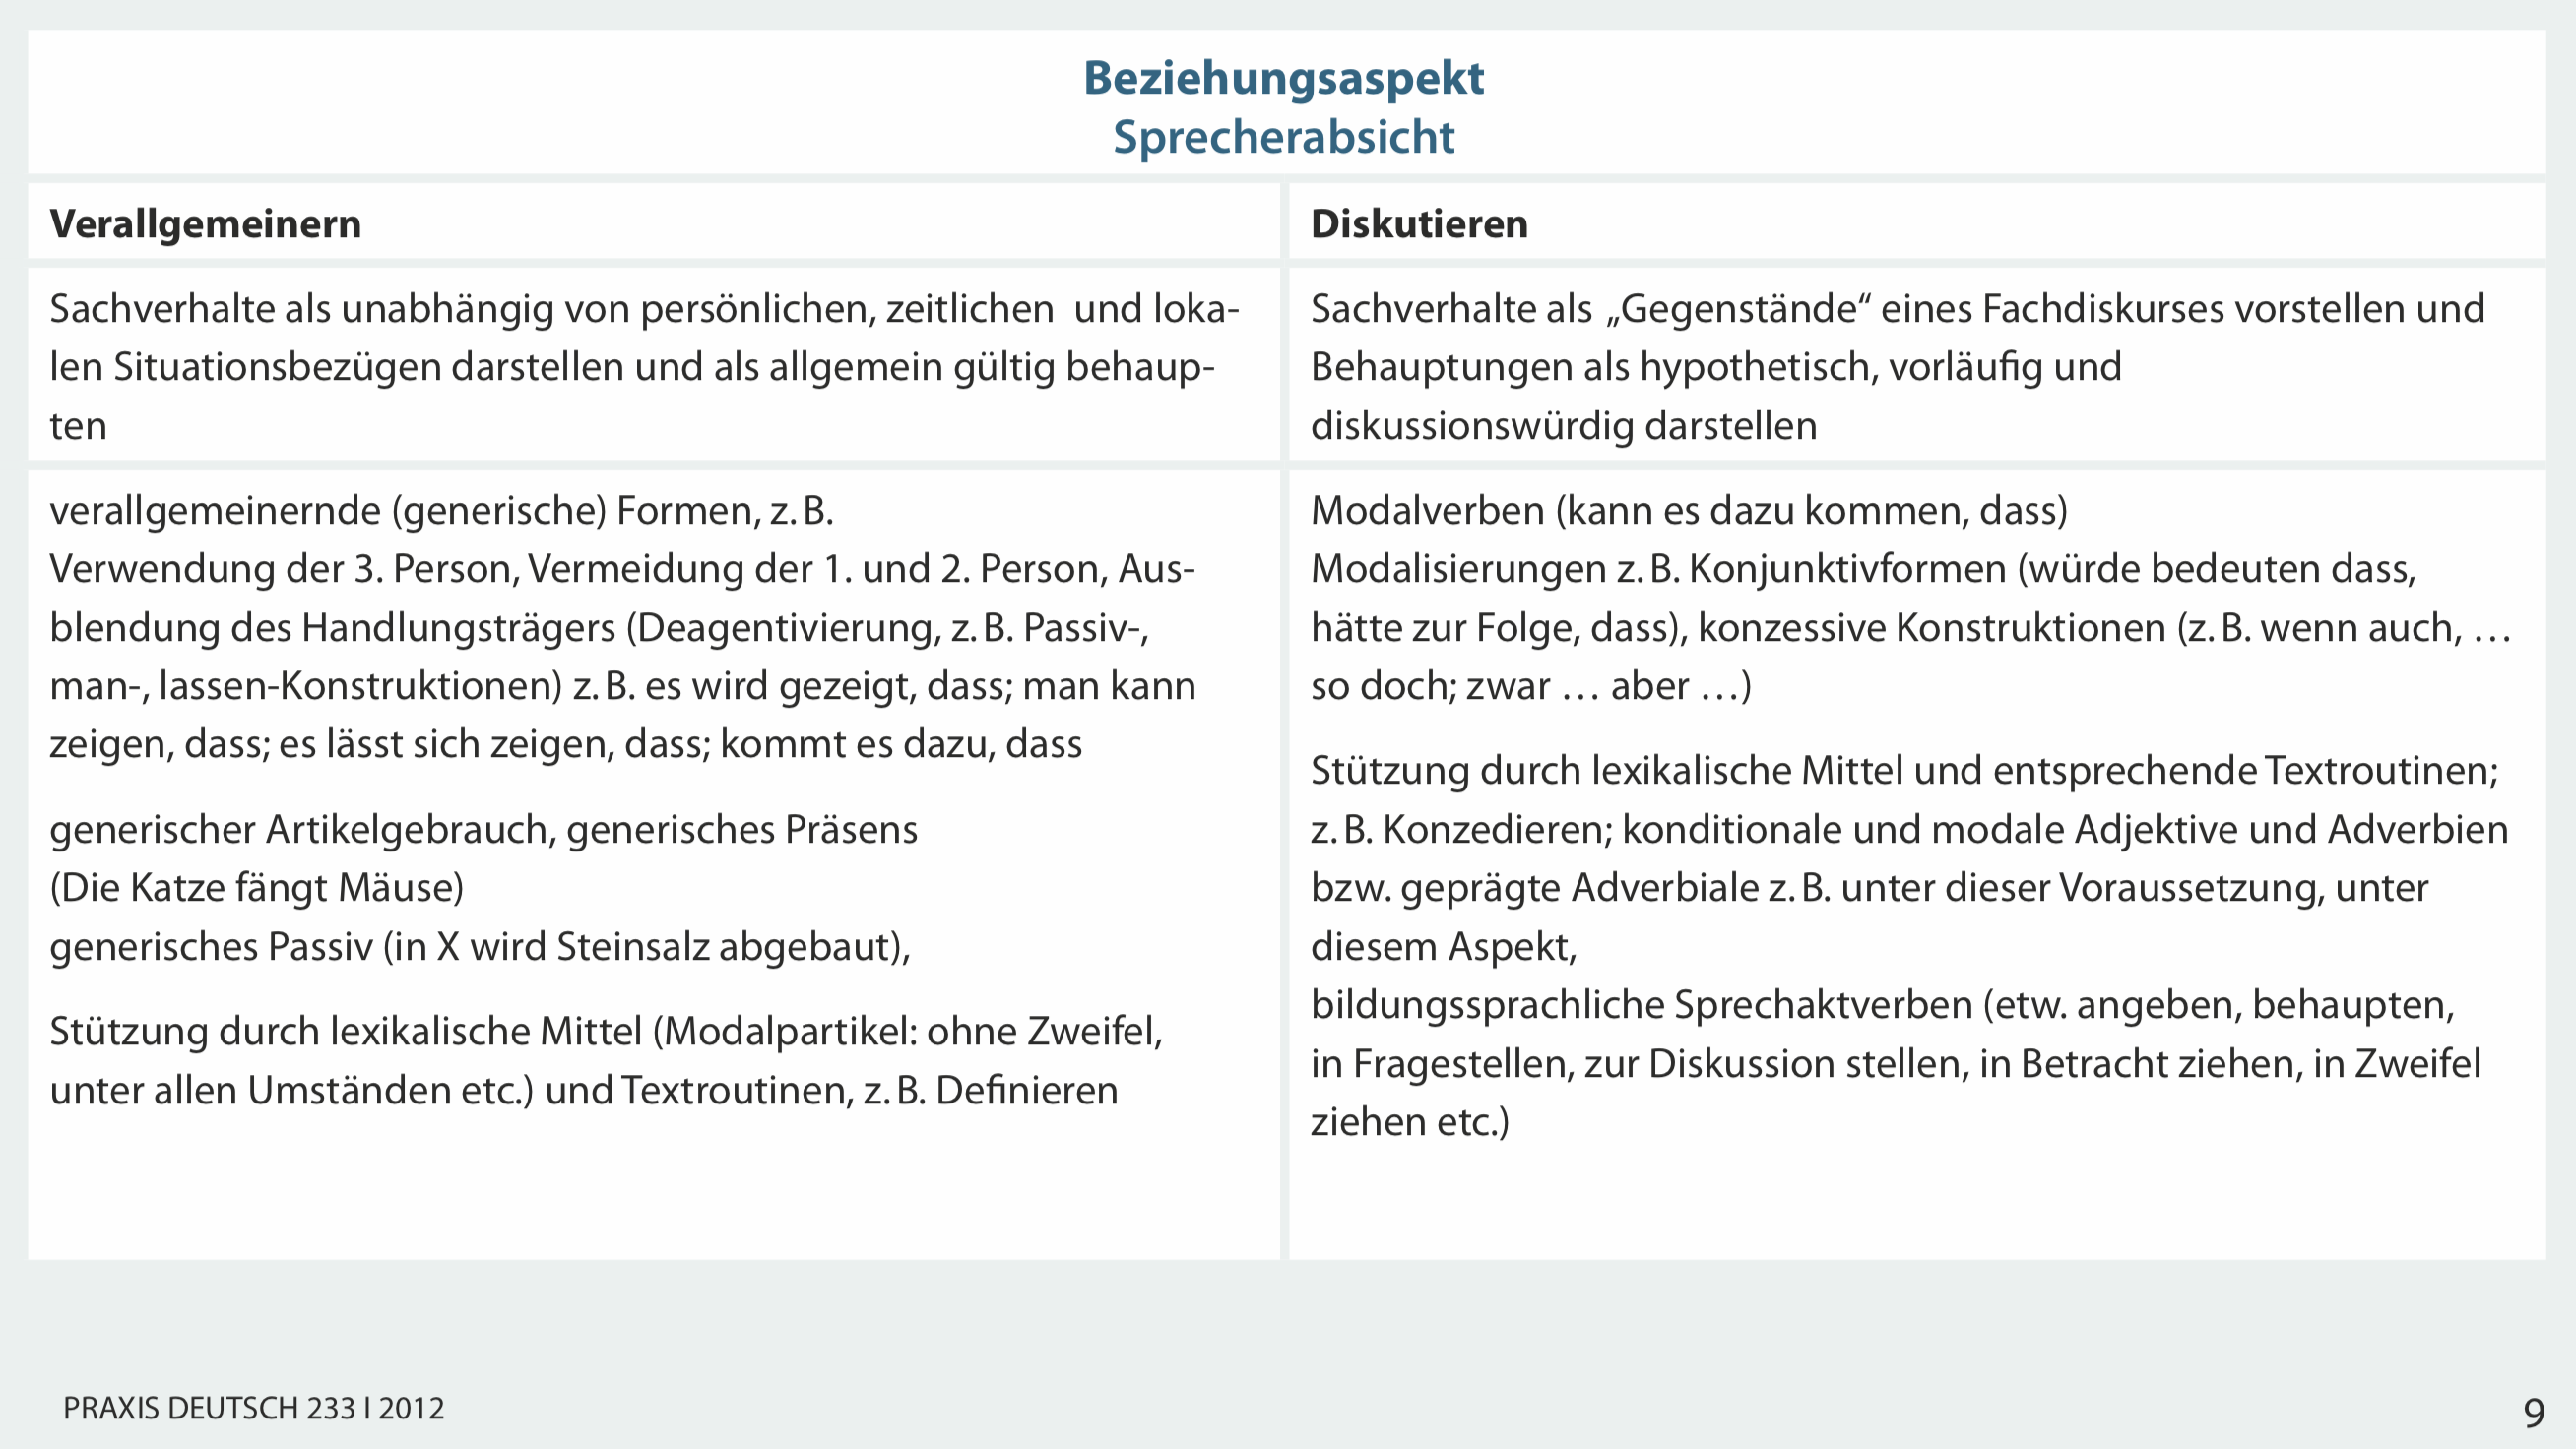
\includegraphics[width=0.8\textwidth]{\GRAPHPATH/feilke2}
\end{frame}

\begin{frame}
  {Übrigens: grammatische Mittel und Bildungssprache}
  Aus \citet{Feilke2012}\\
  \Halbzeile
  \centering
  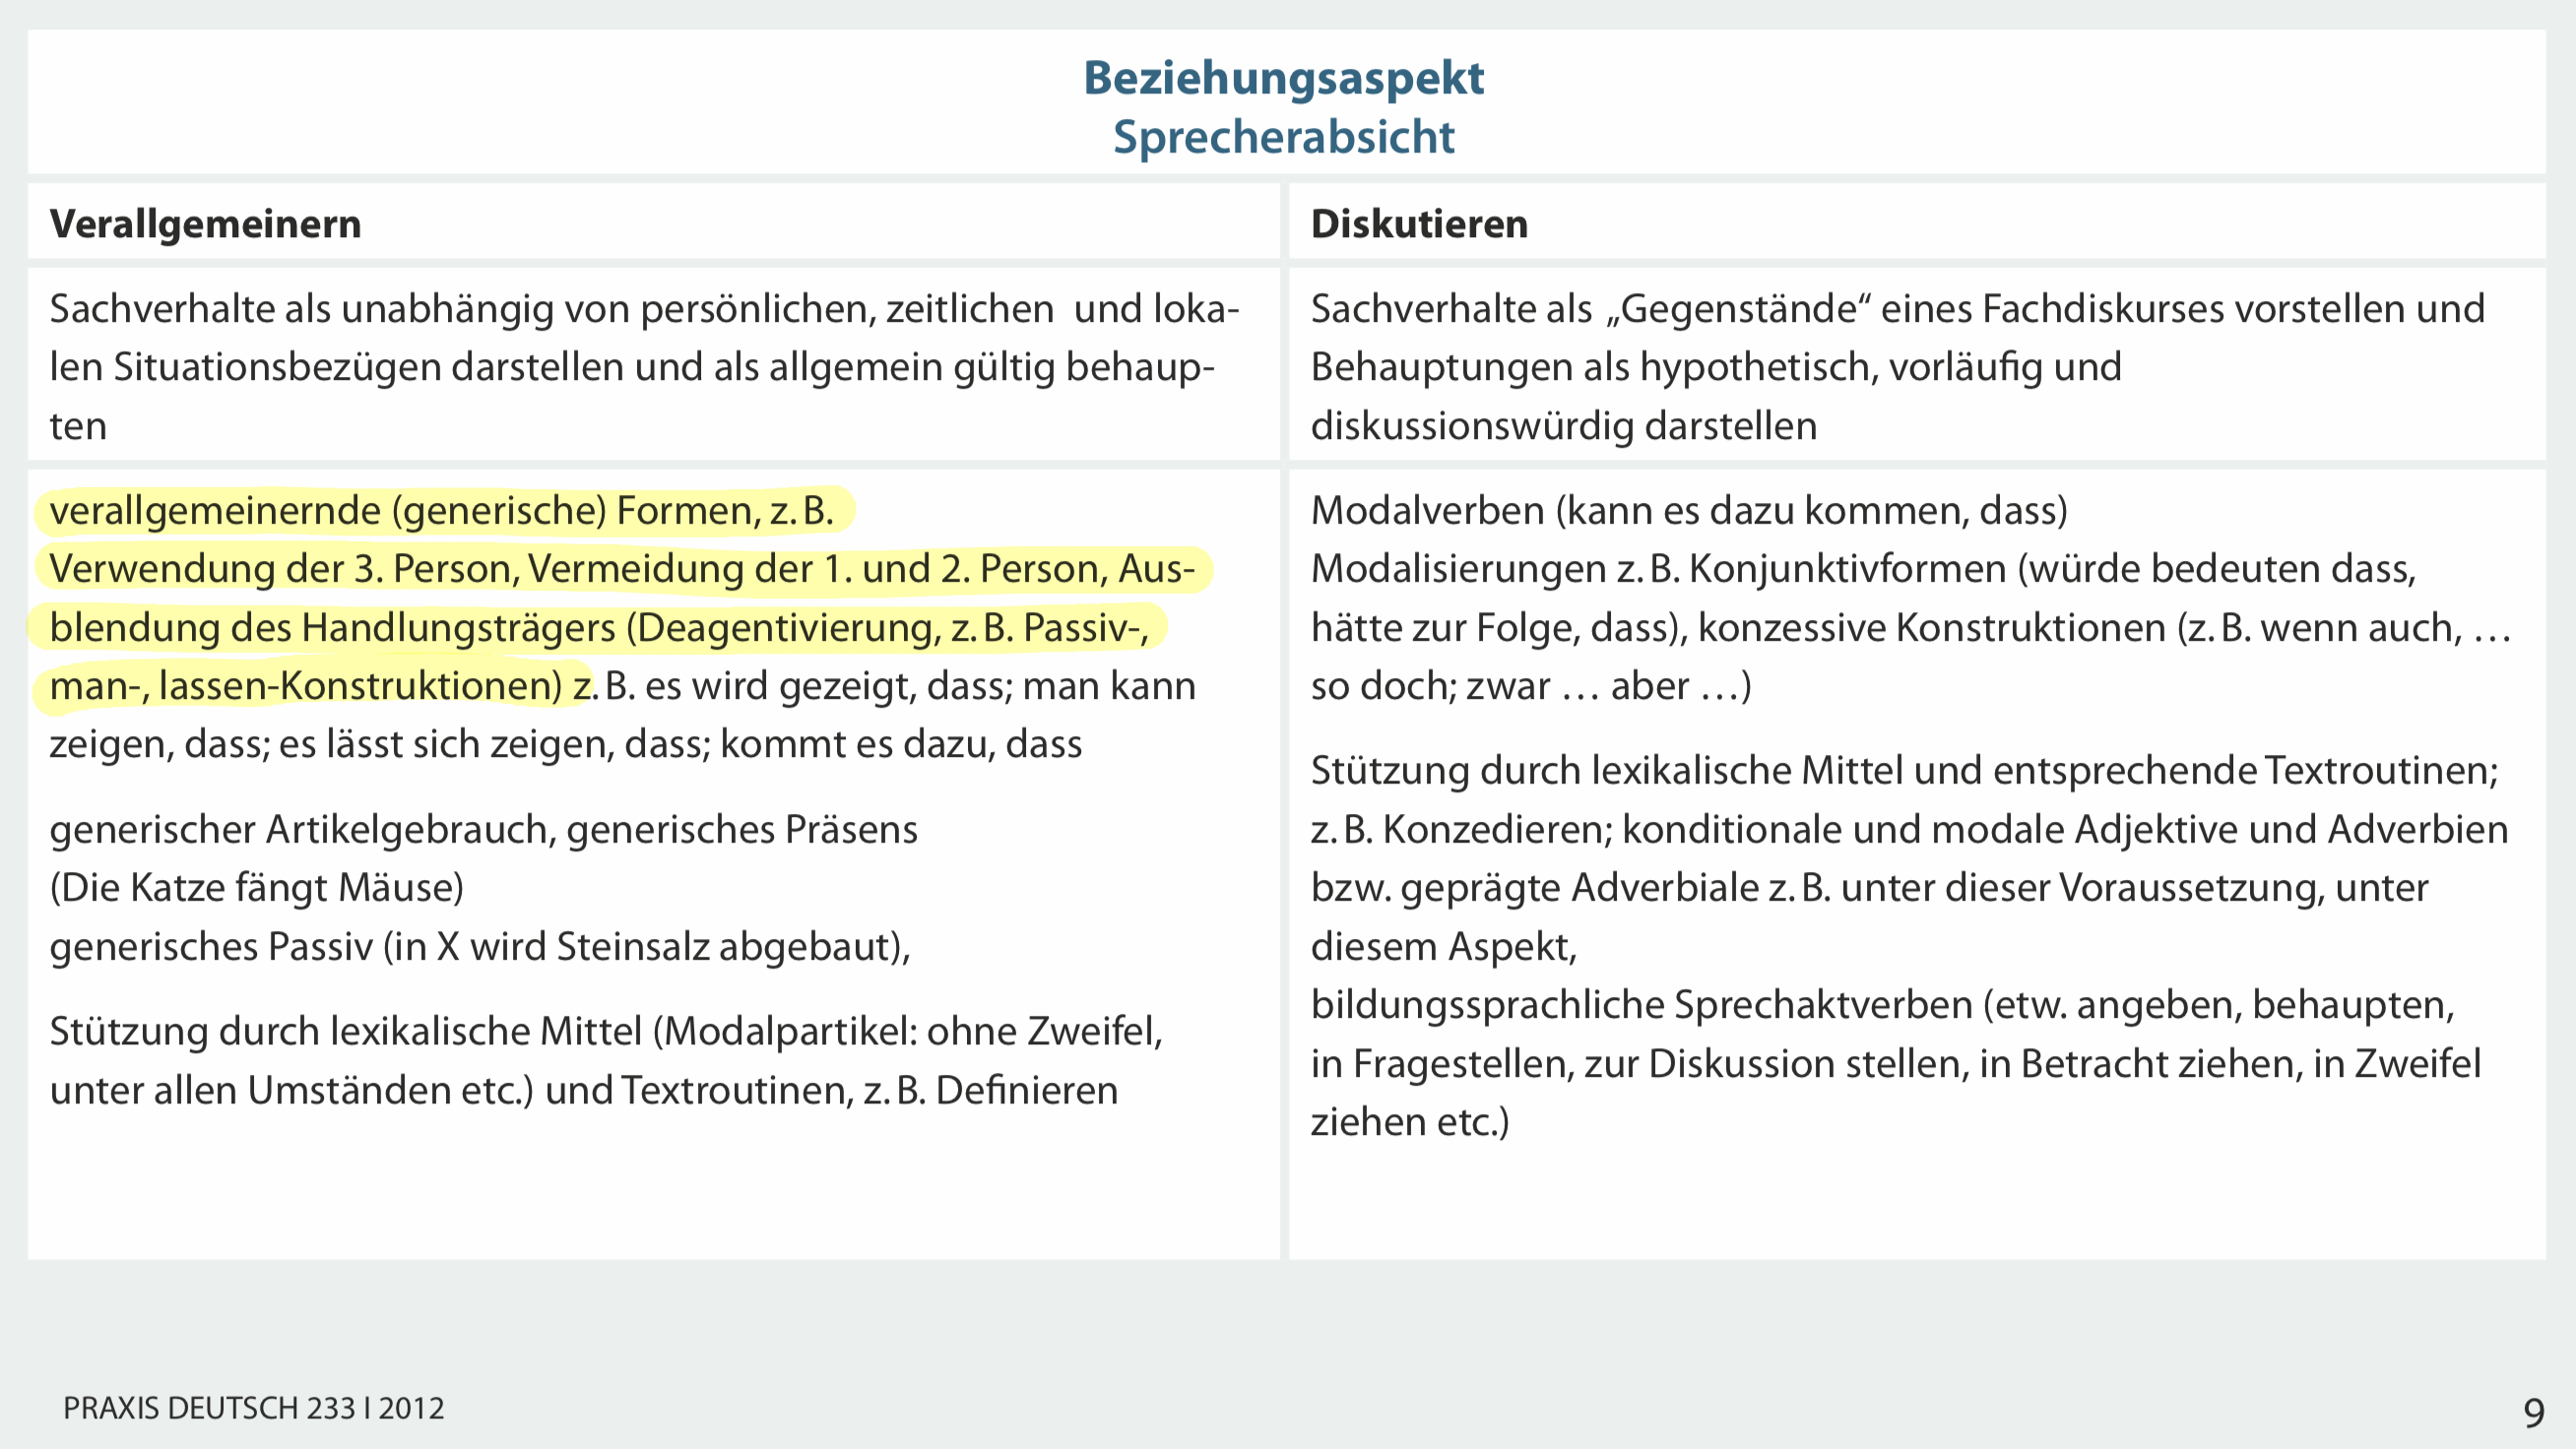
\includegraphics[width=0.8\textwidth]{\GRAPHPATH/feilke2a}
\end{frame}

\begin{frame}
  {Übrigens: grammatische Mittel und Bildungssprache}
  Aus \citet{Feilke2012}\\
  \Halbzeile
  \centering
  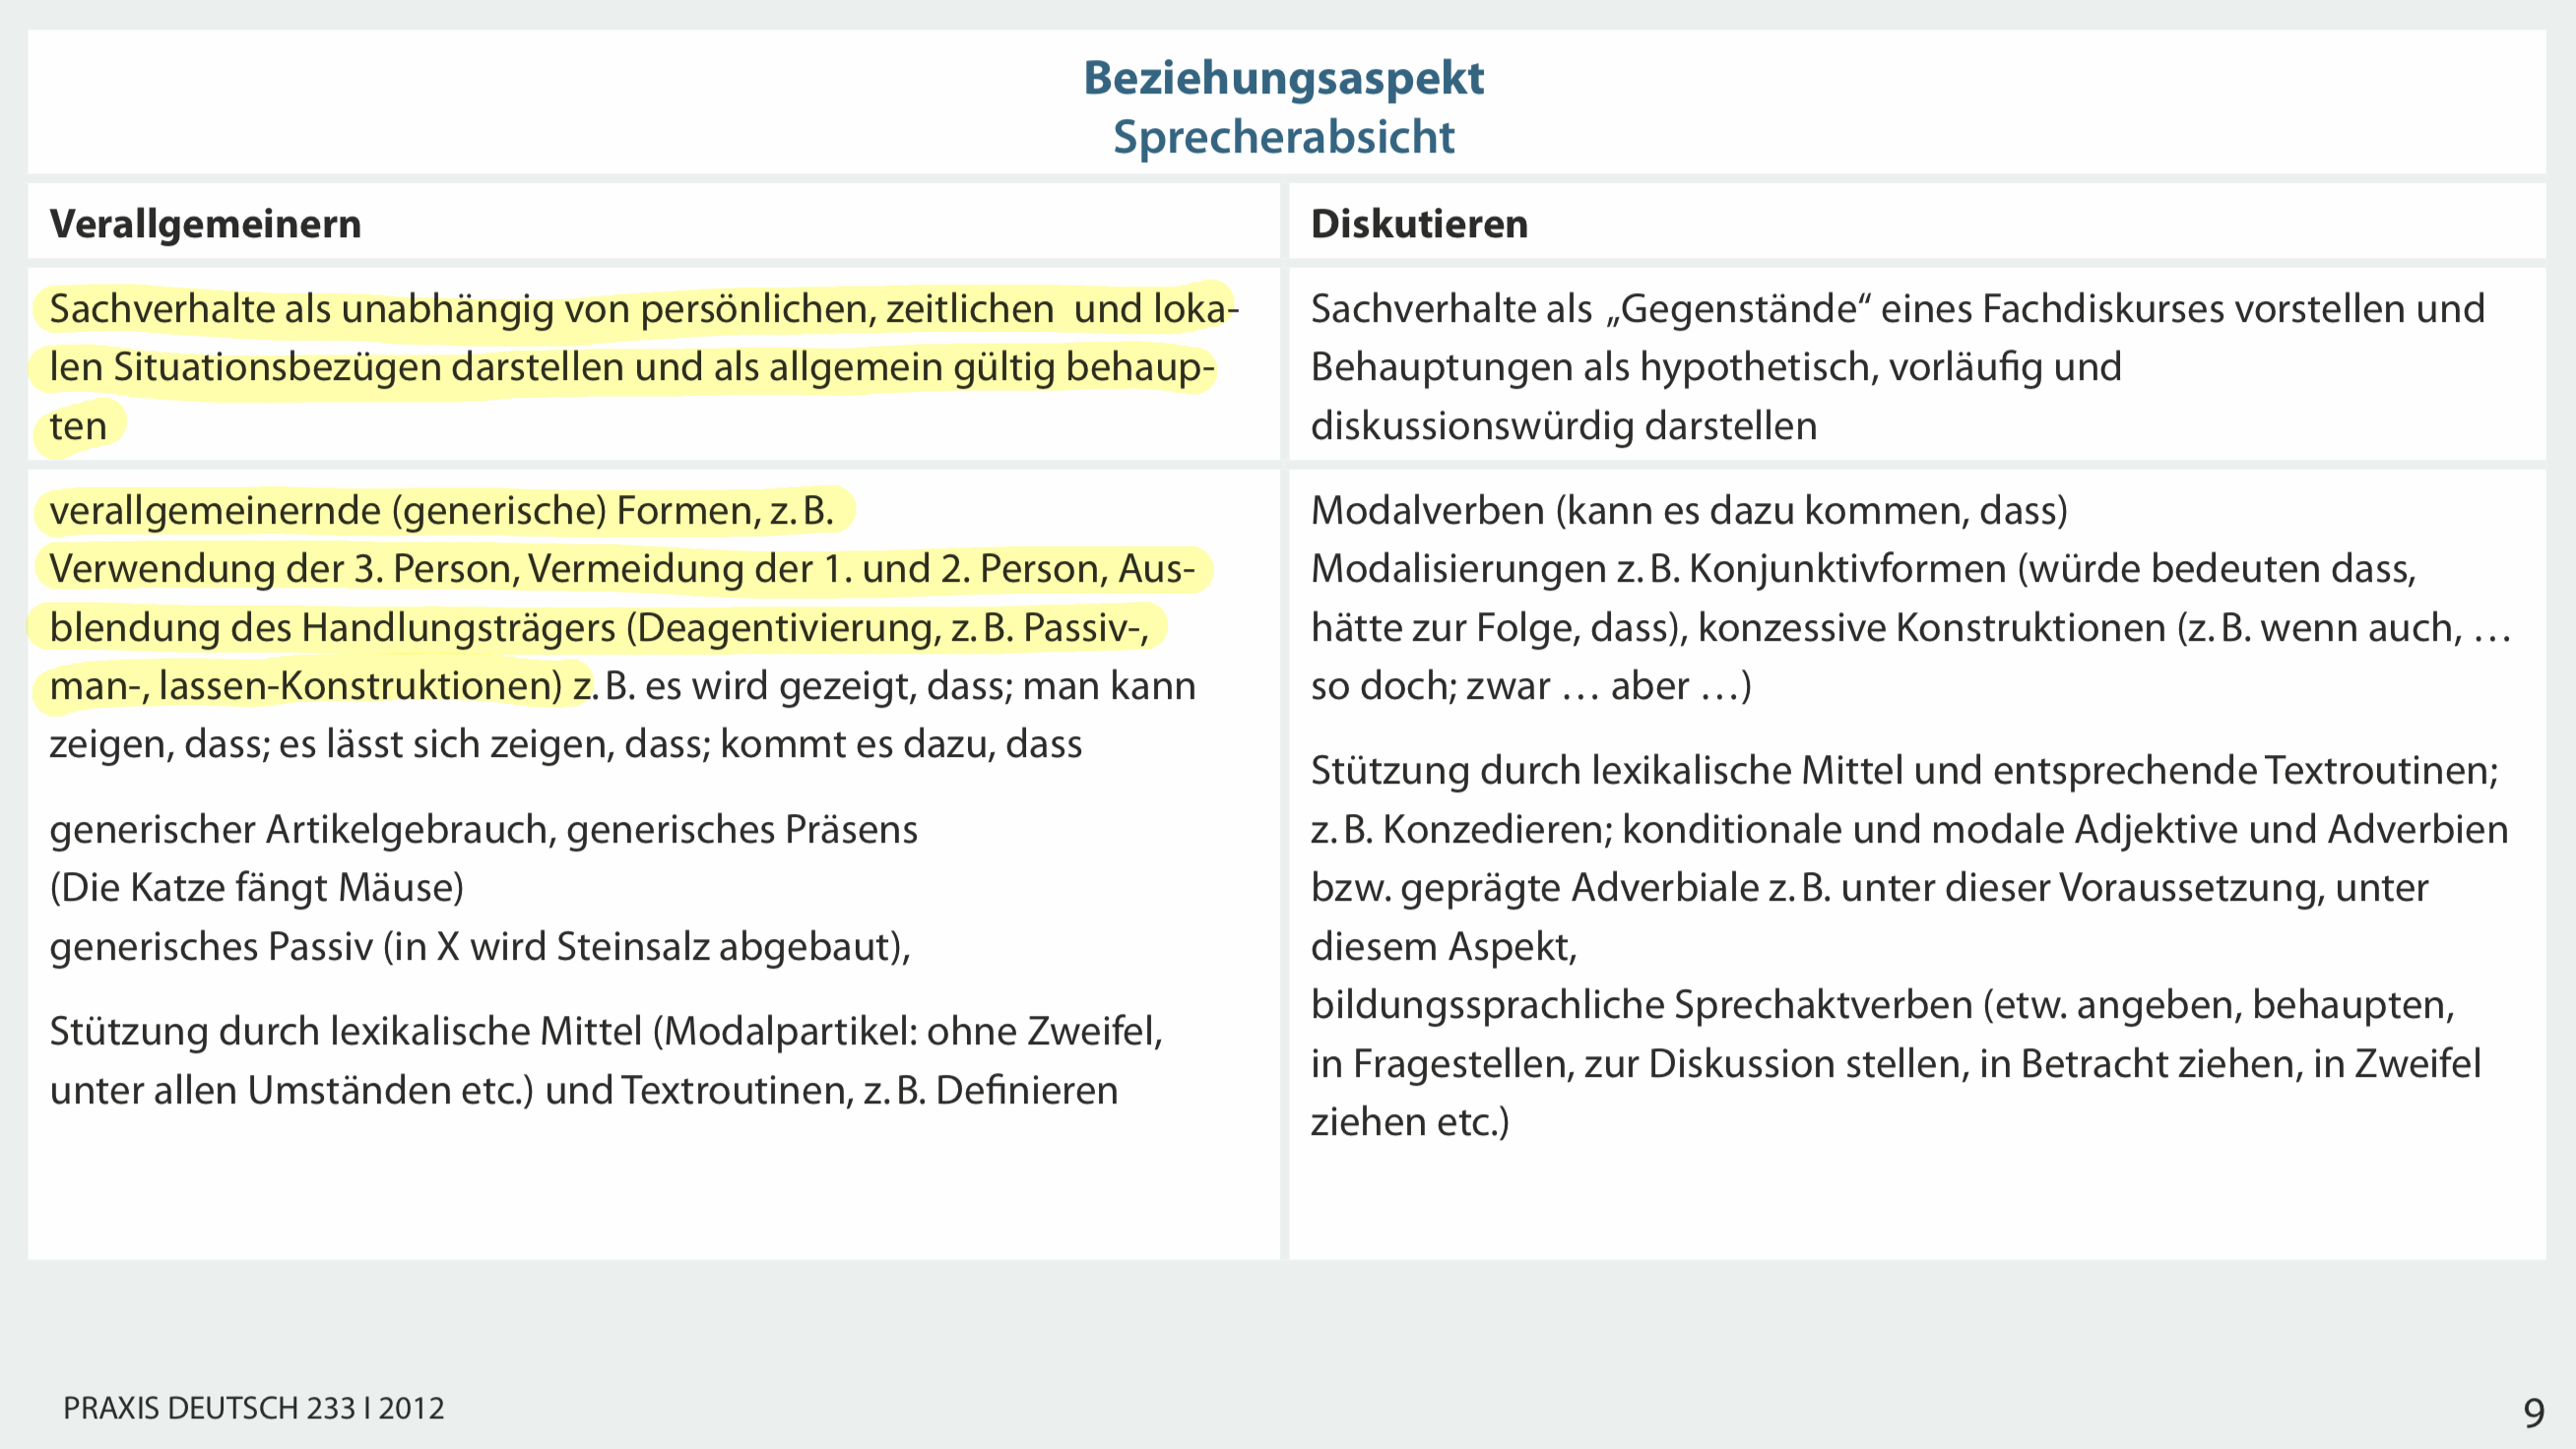
\includegraphics[width=0.8\textwidth]{\GRAPHPATH/feilke2b}
\end{frame}

\begin{frame}
  {Zugabe: Die Kunst der Beispielwahl}
  \pause
  Fehlgriffe beim \alert{Passiv} (\citealt{Gornik2003}, über \citealt{Klotz1995}):\\
  \Zeile
  \pause
  "`Beim Vergleich wird z.\,B.\ auch das Passiv thematisiert (\rot{\textit{Jetzt wird aber sofort ins Bett gegangen}}) und in seiner Wirkung von konkurrierenden Ausdrucksformen abgegrenzt.
  Sich anschließende Untersuchungen zeigen, dass durchaus nicht immer die sog.\ Agensverschweigung als Effekt der Passivnutzung entsteht, sondern im Gegenteil das Agens sogar hervorgehoben werden kann (\orongsch{\textit{Von der damaligen Opposition wurden die Wahlen gewonnen.}})."'\\
  \Halbzeile
  \pause
  \begin{itemize}[<+->]
    \item Probleme?
    \begin{itemize}[<+->]
      \item \rot{unpersönliche Passive} sind atypische Passive
      \item \orongsch{gewinnen} hat wahrscheinlich keine Agensrolle
    \end{itemize}
  \end{itemize}
\end{frame}

\section{Semantische Rollen}

\begin{frame}
  {Semantik-Grammatik-Schnittstelle}
  \pause
  \begin{exe}
    \ex
    \begin{xlist}
      \ex{\alert{Michelle} kauft einen Rottweiler.}
      \pause
      \ex{\alert{Der Rottweiler} schläft.}
      \pause
      \ex{\alert{Der Rottweiler} erfreut Marina.}
    \end{xlist}
  \end{exe}
  \pause
  \Halbzeile
  \begin{itemize}[<+->]
    \item semantische Generalisierung über \alert{Käuferin}, \alert{Schläfer}, \alert{Erfreuer}?
    \item \rot{"`Das Subjekt drückt aus, wer oder was im Satz handelt."'}
    \item Nur die \alert{Käuferin} handelt!
      \Halbzeile
    \item Verben als Kodierung eines \alert{Situationstyps} 
    \item Situationstypen mit charakteristischen \alert{Mitspielern}
    \item Handelnde, Betroffene, Veränderte, Emotionen Erfahrende, \ldots
    \item "`Mitspieler"' im weiteren Sinn, auch Gegenstände, Zeitpunkte usw.
      \Halbzeile
    \item Gleichsetzung von Rollen mit Kasus: \rot{absoluter Unsinn}
  \end{itemize}
\end{frame}

\begin{frame}
  {Agens und Experiencer}
  \pause
  \begin{exe}
    \ex
    \begin{xlist}
      \ex{\alert{Michelle} kauft \orongsch{einen Rottweiler}.}
      \ex{\orongsch{Der Rottweiler} schläft.}
      \ex{\orongsch{Der Rottweiler} erfreut \rot{Marina}.}
    \end{xlist}
  \end{exe}
  \pause
  \Halbzeile
  \begin{itemize}[<+->]
    \item Rollen in den Beispielen
      \begin{itemize}[<+->]
        \item \alert{Michelle}: Handelnde = \alert{Agens}
        \item \rot{Marina}: psychischen Zustand Erfahrende: \rot{Experiencer}
        \item \orongsch{Rottweiler}: andere Rollen, hier nicht weiter analysiert (Rx)
      \end{itemize}
  \end{itemize}
\end{frame}

\begin{frame}
  {Rollenzuweisung\ldots\ und Ergänzungen und Angaben}
  \pause
  \begin{itemize}[<+->]
    \item für einen Situationstyp charakteristische Rollen?
      \Viertelzeile
    \item (fast) \alert{immer} \zB
      \begin{itemize}[<+->]
        \item \alert{Zeitpunkt}
        \item \alert{Ort}
        \item \alert{Dauer}
      \end{itemize}
      \Viertelzeile
    \item \alert{nicht immer} \zB
      \begin{itemize}[<+->]
        \item \rot{Handelnde} (\textit{schlafen}, \textit{fallen}, \textit{gefallen}, \ldots)
        \item \rot{psychischen Zustand Erfahrende} (\textit{laufen}, \textit{reparieren}, \textit{spinnen}, \ldots)
        \item \rot{Veränderte} (\textit{betrachten}, \textit{belassen}, \textit{verkaufe}, \ldots)
      \end{itemize}
      \Viertelzeile
    \item Auch wenn Kaufen, Fallen usw.\ Emotionen auslöst:\\
      \alert{Das jeweilige Verb (\textit{kaufen}, \textit{fallen} usw.) sagt darüber nichts aus!}
      \Viertelzeile
    \item \rot{Ergänzung}: gekoppelt an \alert{verbspezifische} Rolle 
    \item \alert{Angabe}: gekoppelt an \alert{verbunspezifische} Rolle
    \item \textit{(nicht) subklassenspezifische Lizenzierung}
  \end{itemize}
\end{frame}

\begin{frame}
  {Das Prinzip der Rollenzuweisung}
  \pause
  \begin{itemize}[<+->]
    \item situationsspezifische Rollen: \alert{nur einmal vergebbar}\\
    = Prinzip der Rollenzuweisung
      \Halbzeile
    \item semantische Motivation für:
      \begin{itemize}[<+->]
        \item Angaben sind iterierbar,
        \item Ergänzungen nicht.
      \end{itemize}
      \Halbzeile
    \item und \alert{Koordinationen}?
  \end{itemize}
  \pause
  \begin{exe}
    \ex \alert{Marina und Michelle} kaufen bei \rot{einer seriösen Züchterin\\
    und ihrer Freundin} einen \orongsch{Dobermann und einen Rottweiler}.
  \end{exe}
  \pause
  \begin{itemize}[<+->]
    \item semantisch: Summenindividuen o.\,ä.
    \item \alert{Grammatik und Semantik untrennbar, gegenseitig bedingend}
  \end{itemize}
\end{frame}

\section{Subjekte}

\begin{frame}
  {Kernfrage: Brauchen wir den Begriff "`Subjekt"'?}
  \pause
  \textit{"`In jedem vollständigen Satz wird das Prädikat durch das Subjekt ergänzt. Das Subjekt nennt die Person oder die Sache, von der das Geschehen ausgeht, oder zu der ein Zustand gehört."'}\\
  \pause\Viertelzeile
  {\small (Mein Übungsbuch: Grammatik Deutsch im Griff 5.\slash 6.~Klasse, Klett 2018, S.~93)}
  \pause
  \Halbzeile
  \begin{itemize}[<+->]
    \item Na, was sagen wir denn dazu?
      \begin{itemize}[<+->]
        \item \rot{Wetter-Verben}?
        \item \rot{Passivsätze}?
        \item \rot{Subjektsätze}?
        \item \ldots um nur einige der wichtigsten Probleme zu nennen.
      \end{itemize}
  \end{itemize}
\end{frame}

\begin{frame}
  {Potentielle Subjekte: Wo wollen wir denn hin?}
  \pause
  \begin{exe}
    \ex
    \begin{xlist}
      \ex[ ]{\alert{[Frau Brüggenolte]} backt einen Kuchen.}
      \ex[*]{Backt einen Kuchen.}
      \pause
      \ex[ ]{\alert{[Herr Uhl]} raucht.}
      \ex[*]{Raucht.}
      \pause
      \ex[ ]{\alert{[Es]} regnet.}
      \ex[*]{Regnet.}
      \pause
      \ex[ ]{\alert{[Dass Herr Oelschlägel jeden Tag staubsaugt]}, nervt Herrn Uhl.}
      \ex[*]{Nervt Herrn Uhl.}
      \pause
      \ex[ ]{\alert{[Zu Fuß den Fahrstuhl zu überholen]}, machte mir als Kind Spaß.}
      \ex[*]{Machte mir als Kind Spaß.}
      \pause
      \ex[ ]{Es friert mich.}
      \ex[ ]{Mich friert. \onslide<7->{\rot{Ups!}}}
    \end{xlist}
  \end{exe}
  \pause
    Was ist diesen \alert{regierten obligatorischen Ergänzungen} gemein?
\end{frame}

\begin{frame}
  {Subjekte = verbregierte kongruierende Nominative}
  \pause
  \begin{itemize}[<+->]
    \item Was wird denn so alles "`Subjekt"' genannt?
      \begin{itemize}[<+->]
        \item \alert{regierte Nominative}
        \item \alert{die mit dem Verb kongruieren}
        \item oder \alert{Nebensätze} an der Stelle solcher Nominative
        \item \grau{Achtung: Nebensätze haben keine Kongruenzmerkmale\\
            und keinen Kasus! Subjektsätze sind nicht \textit{3.~Person Nominativ}.}
      \end{itemize}
      \Halbzeile
    \item \rot{Das wars. Nichts mit "`Satzgegenstand"', "`Handelnde"' usw.}
      \Halbzeile
    \item Brauchen wir den Begriff dann?
      \begin{itemize}[<+->]
        \item \alert{eigentlich überflüssig}
        \item \ldots aber ganz praktisch als Abkürzung
      \end{itemize}
  \end{itemize}
  \pause
\end{frame}

\section{Expletiva}

\begin{frame}
  {\textit{Es} ist nicht, was es scheint.}
  \pause
  \begin{exe}
    \ex
    \begin{xlist}
      \ex{\alert<4->{Es} öffnet die Tür.}
      \ex{\rot<4->{Es} regt mich auf, dass die Politik schon wieder versagt.}
      \ex{\rot<4->{Es} öffnet ein Kind die Tür.}
      \ex{\rot<4->{Es} wird jetzt gearbeitet.}
      \ex{\rot<4->{Es} friert mich.}
      \ex{\rot<4->{Es} regnet in Strömen.}
    \end{xlist}
  \end{exe}
  \pause
  \begin{itemize}[<+->]
    \item Ersetzbar durch Vollpronomen (\zB\ \textit{dieses})?
    \item \alert{Subjektpronomen}
  \end{itemize}
\end{frame}

\begin{frame}
  {\textit{Es} ist nicht, was es scheint.}
  \begin{exe}
    \ex
    \begin{xlist}
      \ex{\grau{Es öffnet die Tür.}}
      \ex{\alert<3->{Es} regt mich auf, dass die Politik schon wieder versagt.}
      \ex{\rot<3->{Es} öffnet ein Kind die Tür.}
      \ex{\rot<3->{Es} wird jetzt gearbeitet.}
      \ex{\rot<3->{Es} friert mich.}
      \ex{\rot<3->{Es} regnet in Strömen.}
    \end{xlist}
  \end{exe}
  \pause
  \begin{itemize}[<+->]
    \item Tritt auf mit und korreliert mit Subjektsatz?
    \item \alert{Korrelat}
  \end{itemize}
\end{frame}

\begin{frame}
  {\textit{Es} ist nicht, was es scheint.}
  \begin{exe}
    \ex
    \begin{xlist}
      \ex{\grau{Es öffnet die Tür.}}
      \ex{\grau{Es regt mich auf, dass die Politik schon wieder versagt.}}
      \ex{\alert<4->{Es} öffnet ein Kind die Tür.}
      \ex{\alert<4->{Es} wird jetzt gearbeitet.}
      \ex{\rot<4->{Es} friert mich.}
      \ex{\rot<4->{Es} regnet in Strömen.}
    \end{xlist}
  \end{exe}
  \pause
  \begin{itemize}[<+->]
    \item Immer in Satz-Erst-Position (\textit{Vorfeld})?
    \item \ldots und immer weglassbar
    \item \alert{positionales \textit{Es}} oder \alert{Vorfeld-\textit{Es}}
    \item reiner Vorfeld-Füller
  \end{itemize}
\end{frame}

\begin{frame}
  {\textit{Es} ist nicht, was es scheint.}
  \begin{exe}
    \ex
    \begin{xlist}
      \ex{\grau{Es öffnet die Tür.}}
      \ex{\grau{Es regt mich auf, dass die Politik schon wieder versagt.}}
      \ex{\grau{Es öffnet ein Kind die Tür.}}
      \ex{\grau{Es wird jetzt gearbeitet.}}
      \ex{\alert<3->{Es} friert mich.}
      \ex{\orongsch<4->{Es} regnet in Strömen.}
    \end{xlist}
  \end{exe}
  \pause
  \begin{itemize}[<+->]
    \item Optional?
    \item Ja: \alert{fakultative Ergänzung bei \textit{Experiencer}-Verben}
    \item Nein: \orongsch{obligatorische Ergänzung bei \textit{Wetter}-Verben}
      \Halbzeile
    \item Achtung: Die Ergänzung ist hier absolut festgelegt auf \textit{es}!
    \item Es wird nicht nur der Kasus oder die PP-Form regiert.
  \end{itemize}
\end{frame}


\section{Prädikate}

\begin{frame}
  {"`Satzprädikat"'?}
  \pause
  \textit{"`Jeder vollständige Satz besitzt (sic!) ein Prädikat. Es drückt aus, was im Satz geschieht oder ist. Das Prädikat ist der wichtigste Bestandteil eines Satzes. Von ihm hängen die anderen Bausteine des Satzes ab. [\ldots] Das Prädikat ist immer eine konjugierte Verbform."'}\\
  \pause\Viertelzeile
  {\small (Mein Übungsbuch: Grammatik Deutsch im Griff 5.\slash 6.~Klasse, Klett 2018, S.~90)}
  \pause
  \Halbzeile
  \begin{itemize}[<+->]
    \item \rot{Unterschied zwischen \textit{Prädikat} und \textit{finites Verb}?}
    \item analytische Verbformen (\textit{geklebt haben durfte})?
    \item "`was geschieht oder ist"'? -- \textit{Chloë spielt Tennis.}
    \item OK, vielleicht ohne Subjekt? -- \textit{spielt Tennis.}
      \Halbzeile
    \item \textit{Prädikat} ist ein \alert{semantischer Begriff} (s.~\textit{Prädikatenlogik})\ldots
    \item \ldots der \alert{in der Schulgrammatik nichts zu suchen hat}.
  \end{itemize}
\end{frame}

\begin{frame}
  {"`Prädikativergänzungen"'}
  \pause
  Andere \textit{prädikative} Konstituenten außer dem \textit{Satzprädikat}?\\
  \Halbzeile
  \begin{exe}
    \ex\label{ex:praedikative022}
    \begin{xlist}
      \ex{\label{ex:praedikative023} Stig wird [gesund].}
      \pause
      \ex{\label{ex:praedikative024} Stig bleibt [ein Arzt].}
      \pause
      \ex{\label{ex:praedikative025} Stig ist, [wie er ist].}
      \pause
      \ex{\label{ex:praedikative026} Stig ist [in Kopenhagen].}
    \end{xlist}
  \end{exe}
  \pause
  \Halbzeile
  \begin{itemize}[<+->]
    \item \alert{Prädikativergänzung} bei Kopulaverben
    \item besser \rot{nicht \textit{Prädikatsnomen}} (s.~w-Satz und PP)
    \item Nominative (\textit{ein Arzt}): keine Kongruenz
  \end{itemize}
\end{frame}

\begin{frame}
  {Resultativprädikate}
  \pause
  Sind das "`Adverben"' oder "`Adverbiale"'\ldots oder was?\\
  \Halbzeile
  \pause
  \begin{exe}
    \ex\label{ex:praedikative027}
    \begin{xlist}
      \ex{\label{ex:praedikative028} Er fischt den Teich [leer].
      \onslide<5->{\alert{→ Der Teich wird [leer].}}}
      \ex{\label{ex:praedikative029} Sie färbt den Pullover [grün].
      \onslide<5->{\alert{→ Der Pullover wird [grün].}}}
      \ex{\label{ex:praedikative030} Er stampft die Äpfel [zu Brei].
      \onslide<5->{\alert{→ Die Äpfel werden [zu Brei].}}}
    \end{xlist}
  \end{exe}
  \pause
  \begin{itemize}[<+->]
    \item Als \alert{"`[NP] ist\slash wird [Kopula]."'} formulierbar?
    \item \alert{Ja! Ähnlichkeit zu Prädikativergänzungen bei Kopulaverben.}
    \item "`Resultativprädikate"'?\ldots Meinethalber.
    \item keine einfachen Angaben wegen \rot{Valenzänderung}
    \item also \rot{keine} "`Adverben"', "`adverbiale Bestimmungen"' usw.
  \end{itemize}
\end{frame}

\begin{frame}
  {"`Prädikativergänzungen"'?}
  \pause
  Sind das "`Prädikative"' oder gar "`Prädikatsnomina"'?\\
  \Halbzeile
  \pause
  \begin{exe}
    \ex\label{ex:praedikative032}
    \begin{xlist}
      \ex{\label{ex:praedikative033} Ich halte den Begriff [für unnütz].\\
        \onslide<5->{\rot{→ *Der Begriff ist/wird [für unnütz].}}}
      \ex{\label{ex:praedikative034} Sie gelten bei mir [als Langweiler].\\
        \onslide<5->{\rot{→ *Sie sind/werden [als Langweiler].}}}
      \ex{\label{ex:praedikative035} Das Eis schmeckt [toll].
        \onslide<5->{\rot{→ *Das Eis ist/wird [toll].}}}
    \end{xlist}
  \end{exe}
  \pause
  \begin{itemize}[<+->]
    \item Funktioniert der Kopula-Test?
    \item \rot{Nein! Keine Ähnlichkeit zur Kopulativ-Ergänzung.}
    \item \alert{Form vom Verb vorgegeben}, also:
      \begin{itemize}[<+->]
        \item \textit{für}-PP-Ergänzung (\textit{halten})
        \item \textit{als}-PP(?)-Ergänzung (\textit{gelten})
        \item Adjektiv-Ergänzung (\textit{schmecken}\ldots)\\
          \grau{(Oder Angabe? Siehe evtl.\ Vertiefung~2.2, S.~46.)}
      \end{itemize}
  \end{itemize}
\end{frame}


\section{Vorschau}

